\documentclass[compress]{beamer}
\usepackage{ifthen,verbatim}

\newcommand{\isnote}{}
\xdefinecolor{lightyellow}{rgb}{1.,1.,0.25}
\xdefinecolor{darkblue}{rgb}{0.1,0.1,0.7}

%% Uncomment this to get annotations
%% \def\notes{\addtocounter{page}{-1}
%%            \renewcommand{\isnote}{*}
%% 	   \beamertemplateshadingbackground{lightyellow}{white}
%%            \begin{frame}
%%            \frametitle{Notes for the previous page (page \insertpagenumber)}
%%            \itemize}
%% \def\endnotes{\enditemize
%% 	      \end{frame}
%%               \beamertemplateshadingbackground{white}{white}
%%               \renewcommand{\isnote}{}}

%% Uncomment this to not get annotations
\def\notes{\comment}
\def\endnotes{\endcomment}

\setbeamertemplate{navigation symbols}{}
\setbeamertemplate{headline}{\mbox{ } \hfill
\begin{minipage}{5.5 cm}
\vspace{-0.75 cm} \small
\end{minipage} \hfill
\begin{minipage}{4.5 cm}
\vspace{-0.75 cm} \small
\begin{flushright}
\ifthenelse{\equal{\insertpagenumber}{1}}{}{Jim Pivarski \hspace{0.2 cm} \insertpagenumber\isnote/\pageref{numpages}}
\end{flushright}
\end{minipage}\mbox{\hspace{0.2 cm}}\includegraphics[height=1 cm]{../cmslogo} \hspace{0.1 cm} \includegraphics[height=1 cm]{../tamulogo} \hspace{0.01 cm} \vspace{-1.05 cm}}

\begin{document}
\section*{Title/introduction}

\begin{frame}
\vfill
\begin{center}
\textcolor{darkblue}{\Large Muon Alignment with Tracks}

\vfill
\begin{columns}
\column{0.3\linewidth}
\begin{center}
\large
\textcolor{darkblue}{Jim Pivarski}

\vspace{0.2 cm}
Alexei Safonov
\end{center}

\column{0.3\linewidth}
\begin{center}
\large
K\'aroly Banicz
\end{center}

\column{0.3\linewidth}
\begin{center}
\large
Jim Bellinger
\end{center}
\end{columns}

\begin{columns}
\column{0.3\linewidth}
\begin{center}
\scriptsize
{\it Texas A\&M University}
\end{center}

\column{0.3\linewidth}
\begin{center}
\scriptsize
{\it US-CMS}
\end{center}

\column{0.3\linewidth}
\begin{center}
\scriptsize
{\it University of Wisconsin}
\end{center}
\end{columns}

\vfill
 8 December, 2008

\end{center}
\end{frame}

%% \begin{notes}
%% \item This is the annotated version of my talk.
%% \item If you want the version that I am presenting, download the one
%% labeled ``slides'' on Indico (or just ignore these yellow pages).
%% \item The annotated version is provided for extra detail and a written
%% record of comments that I intend to make orally.
%% \item Yellow notes refer to the content on the {\it previous} page.
%% \item All other slides are identical for the two versions.
%% \end{notes}

\small

\begin{frame}
\frametitle{Summary/Outline}
\begin{itemize}\setlength{\itemsep}{0.25 cm}
\item CSC Overlaps procedure in beam-halo data
\begin{itemize}
\item Reached 300~$\mu$m accuracy!
\item Verified with photogrammetry
\item Everything makes sense in MC
\item Led to the discovery of a 10~$\mu$m (compounded) error in the geometry description
\end{itemize}

\item A first look at layer alignment with CSC Overlaps

\item Wheel/disk alignment in CRAFT
\begin{itemize}
\item Delivered a working system on time
\item Diagnostic of results: dependence on tracker, $\vec{B}$ error
\item Using muon residuals to measure bulk tracker misalignment
\end{itemize}

\item Update on database comparison tool and \mbox{photogrammetry database\hspace{-1 cm}}
\end{itemize}
%% \hspace{-0.83 cm} \textcolor{darkblue}{\Large Outline2}
\end{frame}

\section*{CSC Overlaps Alignment}
\begin{frame}
\begin{center}
\Huge \textcolor{blue}{CSC Overlaps Alignment}
\end{center}
\end{frame}

\begin{frame}
\frametitle{Motivation for CSC Overlaps}
\begin{itemize}
\item Baseline alignment procedure shown to require 10--100~pb$^{-1}$ for a few hundred micron precision
\item Quicker alternative:
\begin{enumerate}\setlength{\itemsep}{0.1 cm}
\item relative alignment of chambers in each ring (CSC Overlaps)
\item align whole ring relative to tracker with a small number of quality globalMuon tracks
\end{enumerate}
\item Particularly good for layer alignment
\end{itemize}

\begin{columns}
\column{0.5\linewidth}
Overlaps chamber alignment:
\begin{enumerate}\setlength{\itemsep}{0 cm}
\item select tracks that pass through overlap of chambers in a ring
\item require consistency in pair of segments: slope and intercept
\item solve system
\end{enumerate}

\column{0.2\linewidth}
\includegraphics[width=\linewidth]{overlaps.png}

\column{0.3\linewidth}
\includegraphics[width=\linewidth]{one_station.png}
\end{columns}

\vfill
System is over-constrained: must be consistent with a circle (``closure'')
\end{frame}

\begin{frame}
\frametitle{Three-step procedure}

Interdependencies between alignment parameters are unidirectional

\begin{enumerate}\setcounter{enumi}{-1}
\item Fit segment of track in each chamber to $\phi(z) = a + bz$
\item Align $\varphi_y$ angles (rotation around vertical axis) \hfill $\Delta b \to 0$
\item Align $r\phi$ positions (rotation around beamline) \hfill $\Delta a \to 0$
\item Align $\varphi_z$ angles (rotation in the detector plane) \hfill $d(\Delta a)/dy \to 0$
\end{enumerate}

\begin{columns}
\column{0.35\linewidth}
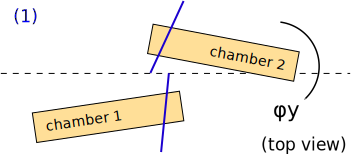
\includegraphics[width=\linewidth]{topview_1.png}
\column{0.01\linewidth}
\hfill $\to$ \hfill
\column{0.35\linewidth}
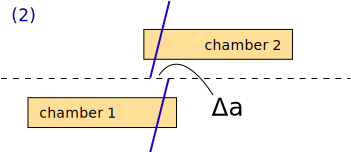
\includegraphics[width=\linewidth]{topview_2.png}
\column{0.01\linewidth}
\hfill $\to$ \hfill
\column{0.25\linewidth}
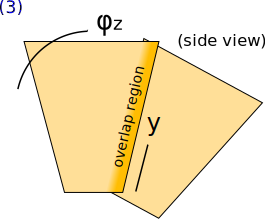
\includegraphics[width=\linewidth]{sideview.png}
\end{columns}

\vfill
\begin{itemize}
\item Parameters decouple when aligned in this order (for example,
  $\varphi_y$ depends only on $\Delta b$, but $r\phi$ depends on
  $\Delta a$ and $\Delta b$)
\item These are all of the rigid-body parameters accessible to \mbox{overlaps tracks\hspace{-1 cm}}
\end{itemize}
\end{frame}

\begin{frame}
\frametitle{Demonstration in Monte Carlo}

\begin{itemize}
\item Randomly misalign chambers and apply procedure using beam-halo Monte Carlo
\begin{itemize}
\item statistics are roughly the same as September beam-halo
\item some chambers have more tracks, others less because $\phi$ distribution not perfectly modeled
\end{itemize}
\item Plot aligned position minus true position in simulation (resolution)
\item Unaligned is grey, aligned is yellow; one histogram entry \mbox{per chamber\hspace{-1 cm}}
\begin{itemize}
\item $\delta \varphi_y \sim 1$~mrad, \hspace{0.2 cm} $\delta r\phi \sim 230$~$\mu$m, \hspace{0.2 cm} $\delta \varphi_z \sim 0.25$~mrad
\end{itemize}
\end{itemize}

\vfill
\begin{columns}
\column{0.33\linewidth}
\includegraphics[width=\linewidth]{mcchamber_phiy.pdf}
\column{0.33\linewidth}
\includegraphics[width=\linewidth]{mcchamber_rphi.pdf}
\column{0.33\linewidth}
\includegraphics[width=\linewidth]{mcchamber_phiz.pdf}
\end{columns}
\end{frame}

\begin{frame}
\frametitle{Alignment in real data}

\vfill
\begin{columns}
\column{0.5\linewidth}
\begin{itemize}
\item Aligned ME$-$2/1 and ME$-$3/1 using beam-halo data
\item Compared with \mbox{photogrammetry\hspace{-1 cm}}
\begin{itemize}
\item only track-based alignment sensitive to $\varphi_y$

(only two alignment pins)
\end{itemize}
\item Plot corrections relative to ideal geometry for \mbox{each chamber\hspace{-1 cm}}
\begin{itemize}
\item track-based: \mbox{solid histogram\hspace{-1 cm}}
\item photogrammetry: \mbox{blue points\hspace{-1 cm}}
\end{itemize}
\item Physical misalignments are $\sim$2~mrad in $\varphi_y$, 1~mm in $r\phi$, and 1~mrad in $\varphi_z$
\item Corrections from independent methods follow each \mbox{other closely\hspace{-1 cm}}
\end{itemize}

\column{0.49\linewidth}
\includegraphics[height=0.95\linewidth, angle=90]{compare_m21_phiy.pdf} \\
\includegraphics[height=0.95\linewidth, angle=90]{compare_m31_x.pdf} \\
\includegraphics[height=0.95\linewidth, angle=90]{compare_m21_phiz.pdf}
\end{columns}

%% \only<1>{\scriptsize Overlay of $r\phi$ translations, track-based and photogrammetry relative to ideal}
%% \only<2>{\scriptsize Overlay of $\varphi_z$ rotations, track-based and photogrammetry relative to ideal}
\end{frame}

\begin{frame}
\frametitle{Determine accuracy from PG}
\begin{itemize}
\item RMS difference between track-based and PG: 340~$\mu$m, 0.42~mrad
\item Photogrammetry $r\phi$ uncertainty is (300/$\sqrt{2}$)~$\mu$m = 210~$\mu$m
\item \textcolor{darkblue}{$r\phi$ errors in track-based method alone} = $\sqrt{340^2 - 210^2} =$ \textcolor{darkblue}{270~$\mu$m}
\item \textcolor{darkblue}{$\varphi_z$ errors} = $\sqrt{0.42^2 - (0.3\cdot\sqrt{2}\mbox{ mm}/1.85\mbox{ m})^2} =$ \textcolor{darkblue}{0.35~mrad}
\end{itemize}

\begin{columns}
\column{0.5\linewidth}
\includegraphics[width=\linewidth]{delta_translations.pdf}
\column{0.5\linewidth}
\includegraphics[width=\linewidth]{delta_rotations.pdf}
\end{columns}
\end{frame}

\begin{frame}
\frametitle{Ring consistency (closure)}
\begin{itemize}
\item Each residual distribution represents the difference in alignment between two chambers
\item Must sum to zero: $(x_1 - x_2) + (x_2 - x_3) + \ldots + (x_N - x_1) = 0$
\item $\varphi_y$ and $\varphi_z$ residuals have always summed to zero (``closed'')
\item $r\phi$ residuals closed in MC, but not in data
\item Agreement with photogrammetry ruled out possibility of alignment
  mistake; pointed to error in CMSSW chamber description
\begin{itemize}
\item active volume of chambers is 2.5~mm closer to beamline, {\it or}
\item active volume is 800~$\mu$m wider than in description
\end{itemize}
\item Oleg found 10~$\mu$m rounding error in strip width description
\begin{itemize}
\item multiplied by $\sim$80 strips $\approx$ 800~$\mu$m wider active volume
\end{itemize}
\item Implemented correction; ME$-$2/1, $-$3/1 closure is now perfect!

\begin{center}
\hspace{-1 cm} $\displaystyle \sum_{\mbox{\scriptsize chamber }i} (r\phi_i - r\phi_{i+1})$ \hspace{0.3 cm}
\begin{tabular}{c c c}
& before (mm) & after (mm) \\\hline
ME$-$2/1 & $+$14.30 & -0.72 $\pm$ 0.42 \\
ME$-$3/1 & $+$15.90 & -0.36 $\pm$ 0.51 \\
\end{tabular}
\end{center}

\end{itemize}
\end{frame}

\begin{frame}
\frametitle{CSC Overlaps conclusions}
\begin{itemize}\setlength{\itemsep}{0.35 cm}
\item Reached goal for ME2,3,4/1 accuracy in real data
\item Routine algorithm can align any ring except ME3/1 (no overlaps)
\begin{itemize}\setlength{\itemsep}{0.15 cm}
\item requested new CSCOverlapsAlignmentAlgorithm package \mbox{in CVS\hspace{-1 cm}}
\item important for rings to be complete (no missing chambers):
  possible to work around a missing chamber by applying external
  constraints (e.g.\ straight line monitors)
\end{itemize}
\item Triggers and AlCa paths defined to collect overlaps events from beam-halo and first collisions
\begin{itemize}\setlength{\itemsep}{0.15 cm}
\item Collisions muons will provide more uniform $\phi$ and $R$ coverage
\item Very little data needed: this 300~$\mu$m resolution comes from 9~minutes of beam-halo!
\end{itemize}
\end{itemize}
\end{frame}

\section*{Early Look at CSC Layers}
\begin{frame}
\begin{center}
\Huge \textcolor{blue}{Early Look at CSC Layers}
\end{center}
\end{frame}

\begin{frame}
\frametitle{CSC layer alignment}

\begin{itemize}
\item {\it First} first look at layer alignment by Karoly in MTCC
\item Internal chamber data can only simultaneously determine four
  layers and a straight track, insensitive to shear
\begin{itemize}
\item method of fixing track to layers 1 and 6:
\end{itemize}

\vspace{-0.5 cm}
\mbox{ } \hfill \includegraphics[width=0.65\linewidth]{layer_alignment_skew.png} \hfill \mbox{ }

\item Overlap events allow us to add one degree of freedom per chamber
\begin{itemize}
\item five layers is enough to describe complete internal alignment
\end{itemize}

\mbox{ } \hfill \includegraphics[width=0.65\linewidth]{layer_alignment_noskew.png} \hfill \hfill \hfill \mbox{ }

\end{itemize}
\end{frame}

\begin{frame}
\frametitle{Plots of layer residuals}

Test in \textcolor{darkblue}{Monte Carlo} with 36$\times$ statistics (folded all pairs)

\vspace{-0.15 cm}
\begin{itemize}
\item residuals (blue points) reproduce misalignment pattern (histogram)
\end{itemize}

\mbox{ } \hfill \includegraphics[height=0.8\linewidth, angle=90]{layer_test.pdf} \hfill \mbox{ }

Example in \textcolor{darkblue}{data}: chamber 7, layer 1 and chamber 8, layer 6 are fixed

\mbox{ } \hfill \includegraphics[height=0.8\linewidth, angle=90]{layer_data.pdf} \hfill \mbox{ }

\end{frame}

\begin{frame}
\frametitle{Typical scale and resolution}

\vspace{0.1 cm}
\begin{columns}
\column{0.6\linewidth}
\begin{itemize}
\item Observed $\sim$100~$\mu$m \mbox{layer misalignments\hspace{-0.25 cm}} in ME$-$2/1 and $-$3/1
\begin{itemize}
\item technique requires chambers to be previously aligned
\item (and must be followed by a chamber re-alignment)
\end{itemize}
\item About half as large as misalignments observed in MTCC
  \mbox{(which was ME$+$)\hspace{-1 cm}}
\item Resolution with full beam-halo run is 40--100~$\mu$m, hard to see misalignments
\end{itemize}

\column{0.4\linewidth}
\includegraphics[width=\linewidth]{layer_hist.pdf}
\end{columns}

\vspace{0.1 cm}
\hspace{-0.45 cm} \begin{minipage}{0.9\linewidth}
\begin{itemize}
\item I have not cross-checked these with FAST measurements yet
\end{itemize}
\end{minipage}

\vspace{0.3 cm}
\hspace{-0.83 cm} \textcolor{darkblue}{\Large Status and conclusions}

\begin{itemize}
\item Not yet integrated into an alignment routine: just illustrative plots
\item Layers only need to be aligned once
\item Definitive CSC layer alignment will probably be done with early \mbox{collisions\hspace{-1 cm}}
\end{itemize}
\end{frame}

\section*{Global Alignment in CRAFT}
\begin{frame}
\begin{center}
\Huge \textcolor{blue}{Global Alignment in CRAFT}
\end{center}
\end{frame}

\begin{frame}
\frametitle{We have globalMuons!}

\begin{columns}
\column{0.5\linewidth}
\begin{itemize}
\item First real-data tests of full baseline HIP procedure:
\begin{itemize}\setlength{\itemsep}{0.05 cm}
\item select globalMuon tracks
\item refit, ignoring muon hits
\item use unbiased residuals to

\mbox{\hspace{-0.5 cm}align} wheels/disks/chambers
\end{itemize}
\end{itemize}

\column{0.6\linewidth}
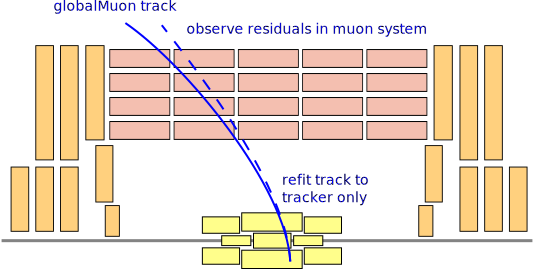
\includegraphics[width=\linewidth]{globalMuons.png}
\end{columns}

\begin{columns}
\column{1.12\linewidth}
\begin{itemize}\setlength{\itemsep}{0.35 cm}
\item Features of CRAFT
\begin{itemize}\setlength{\itemsep}{0.05 cm}
\item 10s--100s of thousands of globalMuons in barrel
\item thousands in endcap
\item magnetic field to select high momentum, minimize alignment errors \\ due to $\vec{B}$-field error and multiple scattering
\end{itemize}

\item Delivered a functional workflow and constants in time for CRAFT re-reco
\begin{itemize}
\item but constants not fully understood, not used in this re-reco
\end{itemize}
\end{itemize}
\end{columns}
\end{frame}

\begin{frame}
\frametitle{Momentum cut/extrapolation}

\begin{columns}
\column{0.6\linewidth}
\begin{itemize}
\item $\vec{B}$-field errors and multiple scattering affect low-momentum tracks
\item Alignment error $\to$ 0 as $|p| \to \infty$
\item Plot vs.\ curvature ($q/p_T$), fit around 0

\vspace{-0.2 cm}
\begin{itemize}
\item constant = misalignment
\item antisymmetric in $q$ = $\vec{B}$ errors
\item symmetric in $q$ = scattering
\end{itemize}
\end{itemize}

\vfill
\begin{columns}
\column{0.5\linewidth}
\includegraphics[width=\linewidth]{residuals_barrel.pdf}
\column{0.58\linewidth}
\includegraphics[width=\linewidth]{residuals_endcap.pdf}
\end{columns}

\begin{tabular}{p{0.5\linewidth} p{0.58\linewidth}}
\scriptsize Barrel wheel 0 & \scriptsize Endcap disk $+$2
\end{tabular}

\column{0.4\linewidth}
\includegraphics[height=\linewidth, angle=90]{qoverpt.pdf}

\includegraphics[width=\linewidth]{oprof_whm2_withcut.pdf}

\mbox{ } \hfill \scriptsize Barrel wheel $-$2 \hfill \mbox{ }

\end{columns}
\end{frame}

\begin{frame}
\frametitle{Measuring the $\vec{B}$-field (aside)}

\vspace{0.2 cm}
\begin{columns}
\column{0.4\linewidth}
\begin{minipage}{1.5\linewidth}
\begin{itemize}\setlength{\itemsep}{0.2 cm}
\item A method like this can also be used to measure the CMS $\vec{B}$-field
\item ``$\phi_z$ residual'' ($\approx$ local $x$ residual divided by $R$) is most
  influenced by $\vec{B}$-field error at $\eta=0$
\item Can derive $\approx$ 0.0035~T (0.1\%) error from slope of
  wheel~0 alignment plot

\begin{minipage}{0.65\linewidth}
\begin{itemize}
\item \mbox{average scale correction through\hspace{-2 cm}} all stations

\item demonstration of statistical power
\end{itemize}

\item 10\% $\vec{B}$-error observed between stations 3 and 4 in a more focused
  study (Ugo Gasparini)
\end{minipage}

\item \mbox{(Large $\vec{B}$-error in a small region is suppressed by $\ell$ in the alignment plot)\hspace{-8 cm}}
\end{itemize}

\end{minipage}

\column{0.6\linewidth}
\hfill \includegraphics[width=0.666\linewidth]{phizresid_profile_pol2fit.pdf}

\vspace{0.5 cm}
\includegraphics[width=\linewidth]{from_p1_to_B.png}

\vspace{0.2 cm}
\mbox{ }
\end{columns}
\end{frame}

\begin{frame}
\frametitle{$\phi_z$ alignment results}

\begin{columns}
\column{0.5\linewidth}

\includegraphics[height=\linewidth, angle=90]{alierr_phiz.pdf}

\includegraphics[height=\linewidth, angle=90]{compare_tracker_alignment_phiz.pdf}

\includegraphics[width=\linewidth]{phiresid_from_muon.png}

\column{0.5\linewidth}

\begin{itemize}
\item Aligned $\phi_z$ for all wheels/disks with
  the $q/p_T \to 0$ method

\item Observed a large (2.5~mrad) twist in the minus endcap 

\item Reproducible in all

\vspace{-0.25 cm}
\begin{itemize}
\item stable 3.8~T \mbox{runs (top plot)\hspace{-1 cm}}

\item tracker \mbox{alignments (middle)\hspace{-0.5 cm}} {\scriptsize (CRUZET, CRAFT-HIP, CRAFT-MillePede)}

\item Muon-MillePede: \mbox{same effect\hspace{-1 cm}}
\end{itemize}

\item Divide into smaller bins: \mbox{replace\hspace{-0.5 cm}} wheel~number with $z$~position (bottom plot)

\vspace{-0.25 cm}
\begin{itemize}
\item real misalignment \mbox{indicated\hspace{-0.5 cm}} by discontinuities
\item external bias indicated by variation inside wheels
\end{itemize}

\end{itemize}
\end{columns}
\end{frame}

\begin{frame}
\frametitle{Check for bias from the tracker}

\vspace{0.25 cm}
\begin{columns}
\column{0.4\linewidth}
\textcolor{darkblue}{Normal muon alignment}

\includegraphics[width=\linewidth]{globalMuons_vsmuon.png}

\column{0.4\linewidth}
\textcolor{darkblue}{Tracker study}

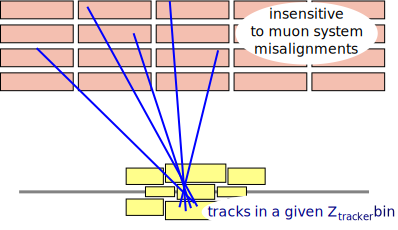
\includegraphics[width=\linewidth]{globalMuons_vstracker.png}
\end{columns}

\begin{itemize}
\item Broad distribution of cosmic rays averages over the detector at the unconstrained part of the track
\end{itemize}

\vspace{-0.6 cm}
\begin{columns}
\column{0.6\linewidth}
\begin{itemize}
\item Plot muon $\phi_z$ residuals vs.\ \mbox{$Z_{PCA}$ (black)\hspace{-1 cm}}
\item Slope (0.2~mrad across TOB) may indicate a twist in the tracker which gets extrapolated to muon system
\item Zijin Guo added a tracker twist \mbox{by hand\hspace{-0.5 cm}} (0.6~mrad, blue points): \mbox{easily observed\hspace{-1 cm}}
\item Need to resolve muon and tracker twists simultaneously
\end{itemize}

\column{0.4\linewidth}
\includegraphics[width=\linewidth]{phiresid_from_tracker_outer_twist2.png}
\end{columns}
\end{frame}

\begin{frame}
\frametitle{$z$ alignment results}

\begin{columns}
\column{0.4\linewidth}
\includegraphics[width=\linewidth]{zresid_from_muon.png}

\column{0.6\linewidth}
\begin{itemize}
\item Effect is large and negative: globalMuons think that the real
  CMS is {\it wider} than ideal geometry by 14~mm across barrel (0.2\%)
\end{itemize}

\vspace{0.5 cm}

\end{columns}

\vspace{-1 cm}
\begin{columns}
\column{0.6\linewidth}

\vspace{1 cm}
\begin{itemize}
\item $z$-expansion is a weak mode of the tracker, hard to determine with tracks

\item Unfortunately, muon residuals can't resolve a plausible
  $z$-expansion \\ (black vs.\ blue: 0.1\% tracker stretch)

\item But we can see large displacements of TEC relative to TOB (discontinuity)

\end{itemize}

\column{0.4\linewidth}
\includegraphics[width=\linewidth]{resid_from_tracker_outer_zexpand.png}

\end{columns}
\end{frame}

\begin{frame}
\frametitle{Tracker $z$ alignment study}

\begin{itemize}
\item Tracker displacements are a scale multiple of muon $z$ residual discontinuities, about 10 times smaller (lever arm of propagation)
\item Select parts of the tracker by cutting on $R_{PCA}$ and by removing tracker hits from refit
\end{itemize}

\vfill
\begin{columns}
\column{0.25\linewidth}
\includegraphics[width=\linewidth]{zresid_from_tracker_outerbottom.pdf}

\includegraphics[width=\linewidth]{tracker_map_outerbottom.png}

\column{0.25\linewidth}
\includegraphics[width=\linewidth]{zresid_from_tracker_innerbottom.pdf}

\includegraphics[width=\linewidth]{tracker_map_innerbottom.png}

\column{0.25\linewidth}
\includegraphics[width=\linewidth]{zresid_from_tracker_innertop.pdf}

\includegraphics[width=\linewidth]{tracker_map_innertop.png}

\column{0.25\linewidth}
\includegraphics[width=\linewidth]{zresid_from_tracker_outertop.pdf}

\includegraphics[width=\linewidth]{tracker_map_outertop.png}
\end{columns}
\end{frame}

\begin{frame}
\frametitle{CRAFT conclusions}

\begin{itemize}\setlength{\itemsep}{-0.05 cm}
\item We have the machinery to produce constants (works in MC, \mbox{see CSA08)\hspace{-1 cm}}
\item Now that we have a large collection of tracks with magnetic
  field, we can diagnose real-data effects:

\vspace{-0.1 cm}
\begin{itemize}\setlength{\itemsep}{-0.025 cm}
\item momentum dependent ($\vec{B}$ error, multiple scattering)
\item dependence on tracker alignment
\item propagator/refitter errors?  (not ruled out)
\end{itemize}
\item Comparison with hardware alignment is not the only validation

\vspace{-0.1 cm}
\begin{itemize}
\item many cross-checks are available in track dataset
\end{itemize}

\item Optimal CRAFT alignment would \mbox{include standAloneMuons:\hspace{-1 cm}}

\mbox{ } \hfill 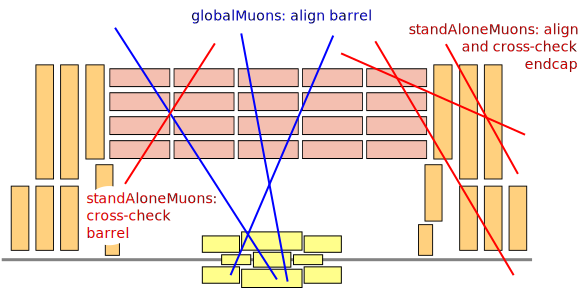
\includegraphics[width=0.7\linewidth]{globalMuons_and_standAloneMuons.png} \hfill \mbox{ }

\item Awaiting cosmic ray-aware standAloneMuon refitter from \mbox{tracking group\hspace{-1 cm}}
\end{itemize}
\end{frame}

\section*{Updates on Tools}
\begin{frame}
\begin{center}
\Huge \textcolor{blue}{Updates on Tools}
\end{center}
\end{frame}

\begin{frame}
\frametitle{Updates on Tools}

\vspace{-1.4 cm}
\begin{columns}
\column{0.3\linewidth}

\vspace{1.7 cm}
\begin{itemize}
\item Database comparison tool (Jim Bellinger)

\begin{minipage}{10 cm}
\begin{itemize}
\item performs {\it local} \\ comparisons of \\ geometry descriptions: i.e.\ matches ME2/1 in geometry A to ME2/1 in geometry B, removing overall translation/rotation, showing only chamber-by-chamber differences
\item complete and in CVS (MuonGeometryArrange)
\end{itemize}
\end{minipage}
\end{itemize}

\column{0.7\linewidth}
\includegraphics[width=\linewidth]{jimb_tool.png}
\end{columns}

\begin{itemize}
\item Conversion of photogrammetry results into CSCAlignmentRcd (Karoly and Oleg)
\begin{itemize}
\item for easier comparison with track-based/hardware alignments (via Jim's tool)
\item for long-term archival
\item most issues resolved: working on $z$ heights of PG targets and sign conventions
\end{itemize}

\end{itemize}
\end{frame}

\section*{Conclusions}

\begin{frame}
\frametitle{Whole-talk conclusions}

\begin{itemize}\setlength{\itemsep}{0.2 cm}
\item The CSC Overlaps procedure really works!
\begin{itemize}
\item we {\it will} be able to align complete rings in 3 d.o.f.\ with desired precision
\item built-in consistency check revealed a geometry error that was quickly fixed
\end{itemize}

\item Overlaps provide a path to CSC layer alignment

\item Baseline alignment workflow is functional, but produces \mbox{puzzling results\hspace{-1 cm}}
\begin{itemize}
\item muon alignment, $\vec{B}$-field commissioning, and tracker alignment, are interrelated but seperable

\item track dataset is rich enough to contain many cross-checks; standAloneMuons will reveal more
\end{itemize}

\item Database comparison tool is ready for use (and is being used)

\item Photogrammetry results will be uploaded to the offline database
\end{itemize}

\label{numpages}
\end{frame}

\end{document}
